% =====================================================================
%  Informe técnico final — Proyecto 1 MCOC (Semana 7)
%  Compilar desde reports/:   pdflatex final.tex   (dos veces, por el índice)
%  Documento en blanco y negro: no se usan colores.
% =====================================================================
\documentclass[11pt,a4paper]{article}

\usepackage[utf8]{inputenc}
\usepackage[T1]{fontenc}
\usepackage{lmodern}
\usepackage[spanish,es-tabla,es-noquoting,es-nodecimaldot]{babel}
\usepackage[a4paper,margin=2.4cm]{geometry}
\usepackage{graphicx}
\usepackage{booktabs}
\usepackage{tabularx}
\usepackage{longtable}
\usepackage{array}
\usepackage{amsmath}
\usepackage{enumitem}
\usepackage[font=small,labelfont=bf]{caption}
\usepackage{listings}
\usepackage{fancyhdr}
\usepackage[htt]{hyphenat}
\usepackage[hidelinks]{hyperref}
\usepackage{textcomp}
\usepackage{float}
\usepackage{newunicodechar}
\newunicodechar{φ}{\ensuremath{\varphi}}
\newunicodechar{‰}{\textperthousand}

\setlist{itemsep=2pt,topsep=4pt}
\setlength{\parskip}{4pt}
\setlength{\parindent}{0pt}
\setlength{\emergencystretch}{3em}
\renewcommand{\arraystretch}{1.12}

\lstset{basicstyle=\ttfamily\small,columns=fullflexible,frame=single,
        breaklines=true,keepspaces=true,showstringspaces=false}

\newcommand{\fecha}{7 de octubre de 2026}

\pagestyle{fancy}
\fancyhf{}
\fancyhead[L]{\small Proyecto 1 MCOC --- Informe técnico final}
\fancyhead[R]{\small Grupo 5}
\fancyfoot[C]{\small\thepage}
\renewcommand{\headrulewidth}{0.4pt}

\graphicspath{{fig/}}

\begin{document}

% ------------------------------------------------------------------ carátula
\begin{titlepage}
\centering
\vspace*{1.2cm}
{\large\scshape Universidad de los Andes\par}
\vspace{0.2cm}
{\normalsize Facultad de Ingeniería y Ciencias Aplicadas --- Ingeniería Civil\par}
\vspace{2.2cm}
\rule{\textwidth}{1.2pt}\par\vspace{0.4cm}
{\LARGE\bfseries Laboratorio estructural digital 3D\\[0.2cm]
Complejo de Ingeniería (Edificios A y B)\par}
\vspace{0.4cm}
{\large OpenSeesPy $\cdot$ Unity $\cdot$ Realidad aumentada\par}
\vspace{0.3cm}\rule{\textwidth}{1.2pt}\par
\vspace{1.4cm}
{\Large Informe técnico final --- Proyecto 1 (Semana 7)\par}
\vspace{2.4cm}
{\large\bfseries Integrantes (Grupo 5)\par}
\vspace{0.3cm}
{\large Nicolás Letelier\par Oscar Rodríguez\par Pablo Arancibia\par}
\vspace{2.0cm}
{\large Curso: Métodos Computacionales en Obras Civiles (MCOC)\par}
\vspace{0.3cm}
{\large \fecha\par}
\vfill
{\small Repositorio: \url{https://github.com/OscarRodriguez17/Proyecto-1-MCOC-Completo}\\
rama \texttt{master}, tag \texttt{entrega-final}\par}
\end{titlepage}

\tableofcontents
\newpage

% =====================================================================
\section{Resumen}

Se construyó un laboratorio estructural digital del Complejo de Ingeniería que
une dos edificios reales de la Universidad, modelados a partir de sus planos
DXF: el \textbf{Edificio A} (planos 2017\_67, hormigón G35, con un anexo y
voladizos metálicos) y el \textbf{Edificio B} (planos 2024\_22, hormigón H30).
Cada edificio es un modelo \textbf{lineal elástico 3D} en OpenSeesPy (6 grados de
libertad por nodo, diafragma rígido por piso, base empotrada) que se analiza en
forma independiente para cinco casos: peso propio y sobrecarga muerta (G),
sobrecarga de uso (Q), su suma (GQ) y sismo pseudoestático en X e Y (EX, EY).

Sobre los resultados verificados se agregó una capa de \textbf{capacidad de
hormigón armado}: un motor de secciones de fibras que entrega curvas
momento--curvatura, diagramas de interacción P--M y la relación
demanda--capacidad (D/C) de cada columna y muro. Todo se exporta a un
\textbf{contrato JSON} único que alimenta un visor en \textbf{Unity} (pre y
postprocesador) y una \textbf{app Android de realidad aumentada} que superpone
los diagramas de esfuerzos de nueve elementos sobre la estructura real.

\begin{table}[h]
\centering
\caption{Cifras principales del modelo final.}
\begin{tabular}{lrr}
\toprule
Magnitud & Edificio A & Edificio B \\
\midrule
Nodos / elementos & 206 / 354 & 235 (+5 maestros) / 350 \\
Peso G [kN] & 45\,417,4 & 48\,171,1 \\
Sobrecarga Q [kN] & 7\,671,3 & 11\,029,6 \\
Corte basal $V = 0{,}10\,W$ [kN] & 4\,541,7 & 4\,817,1 \\
Desplazamiento de techo EX / EY [mm] & 8,48 / 2,35 & 16,00 / 19,77 \\
Deriva máxima de entrepiso EX / EY [‰] & 0,66 / 0,20 & 1,05 / 1,33 \\
Error de equilibrio (5 casos) [kN] & $\le 1{,}1\cdot10^{-9}$ & $\le 3{,}5\cdot10^{-9}$ \\
Superposición, máx.\ $|\Delta R|$ [kN] & $3{,}6\cdot10^{-11}$ & $6{,}0\cdot10^{-11}$ \\
\bottomrule
\end{tabular}
\end{table}

\textbf{Estado de la entrega.} La suite de Python pasa completa
(\textbf{169 tests}) y la de Unity también (\textbf{153 tests} EditMode). El
pipeline completo se volvió a ejecutar desde cero en un entorno limpio con las
versiones fijadas en \texttt{requirements.txt} y reprodujo los archivos de
resultados con el mismo contenido. Las limitaciones que siguen abiertas se declaran
en la sección~\ref{sec:limitaciones}. Entre ellas está un error del motor de
secciones que detectamos en la revisión final: algunos muros largos tienen
puntos de la envolvente P--M con $M = 0$.

% =====================================================================
\section{Edificio e idealización}

\subsection{Los dos edificios}

\textbf{Edificio A} (planos 2017\_67). Retícula de ejes E--J en $x$ (0 a 50~m)
y A3--A1 en $y$ (0 a 16,15~m), con el eje intermedio A2a ($y = 2{,}31$~m).
Tiene una base empotrada a $z = -4{,}21$~m y cuatro losas a $z = -0{,}05$;
3,91; 7,87 y 11,83~m. Pilares de 0,70$\times$0,70~m, vigas V.60/80 y cinco tipos
de muro (ME-32, MI-32, MI-12, M1c-E y M2a). En los dos niveles superiores hay un
anexo metálico entre los ejes I' y J, más un voladizo trasero arriostrado
(ejes G y H) y un voladizo metálico de piso~1 en el eje F. Los elementos de acero
son pilares P.M.~300$\times$300$\times$20, vigas V.M.~300$\times$300$\times$5 y
cuatro diagonales.

\textbf{Edificio B} (planos 2024\_22). Seis niveles con base empotrada a
$z = -4{,}01$~m, cuatro pisos y cubierta a 15,79~m, todos con altura de piso de
3,96~m. Tiene 8 líneas de pilares de 0,70$\times$0,70~m (40 elementos), 60
tramos de muro, vigas V.60/80, V.40/80 y V.30/80 y un bloque de escalera y
ascensor.

\subsection{Idealización común}

\begin{itemize}
  \item Elementos \texttt{elasticBeamColumn} con \texttt{geomTransf Linear} y
        ejes locales explícitos (\texttt{vecxz} no colineal con el eje $i\to j$).
  \item \textbf{Diafragma rígido} por piso
        (\texttt{rigidDiaphragm(3, maestro, *esclavos)} con
        \texttt{constraints Transformation}).
  \item \textbf{Base empotrada}: 23 apoyos en A y 20 en B, todos con
        restricción $[1,1,1,1,1,1]$.
  \item \textbf{Losas no modeladas como elementos}: su peso y su sobrecarga
        llegan a las vigas por áreas tributarias (sección~\ref{sec:cargas}).
  \item \textbf{Vigas T/L} en A: inercia fuerte con ancho efectivo de losa según
        ACI~318-19, Tabla~6.3.2.1. El peso propio de la viga se calcula solo con
        el alma.
  \item \textbf{Muros como columna ancha equivalente}, con su sección real
        ($t \times L$). En A tienen deformación por corte
        ($A_s = 5/6\,A$). En B se unen a las vigas con \textbf{brazos rígidos}
        (35 elementos).
  \item Materiales: G35 en A ($E = 4700\sqrt{35} = 27\,806$~MPa, $\nu = 0{,}2$,
        $\gamma = 25$~kN/m$^3$); H30 en B ($E = 25\,000$~MPa); acero en los
        elementos metálicos de A ($E = 200$~GPa, $\gamma = 78{,}5$~kN/m$^3$).
  \item Cada edificio se \textbf{analiza por separado}, lo que evita el doble
        conteo de áreas tributarias. Un módulo de fusión los reúne en un solo
        contrato JSON, con B desplazado 60~m en $x$ y sus tags renumerados
        (+100\,000).
\end{itemize}

\begin{figure}[h]
\centering
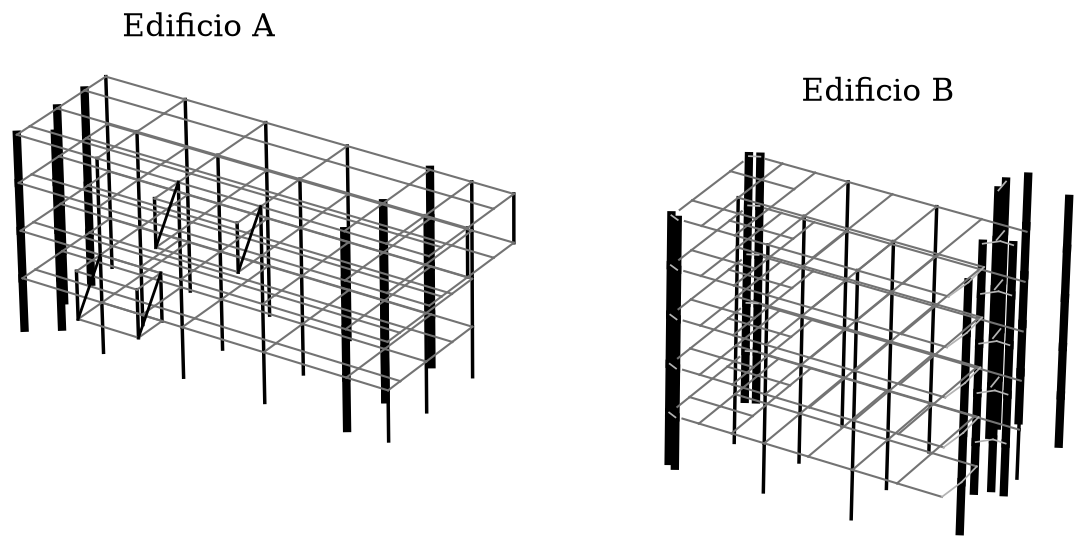
\includegraphics[width=0.95\textwidth]{final_modelo_3d.png}
\caption{Modelo OpenSeesPy de los dos edificios: pilares y muros en negro
(los muros, más gruesos) y vigas en gris.}
\end{figure}

% =====================================================================
\section{Geometría y datos}

\subsection{Extracción desde los planos}

La geometría sale de los DXF con \texttt{ezdxf}. El flujo siempre fue el mismo:
primero se \emph{dibuja} cada lámina para confirmar la lectura y después se
recorren las capas una por una (\texttt{RLE-EJES}, \texttt{RLE-PILAR},
\texttt{RLE-MURO}, \texttt{RLE-VIGA}, \texttt{RLE-PROYECCION} y
\texttt{RLE-TEXTO}). Las coordenadas y cotas verificadas quedan en
\texttt{docs/ficha\_geometria.md} (A), \texttt{docs/ficha\_geometria\_B.md} (B),
\texttt{docs/info\_planos\_dxf.txt} y \texttt{docs/info\_cortes\_elevaciones.txt}.
Los ejes de las vigas de B no caen exactamente sobre los ejes de la grilla, así
que se consolidan con una tolerancia \texttt{GRID\_TOL = 0,30~m}. Sin ese ajuste
quedaban islas de vigas sueltas y la matriz de rigidez resultaba singular.

\subsection{Del modelo base al modelo final (Edificio A)}

El modelo base de A (190 nodos, 321 elementos) se fue ampliando solo con
\textbf{módulos aditivos} que inyectan nodos y elementos con tags nuevos:

\begin{table}[h]
\centering
\caption{Evolución del modelo del Edificio A.}
\begin{tabularx}{\textwidth}{Xrrr}
\toprule
Etapa (módulo) & Nodos & Elementos & G [kN] \\
\midrule
Modelo base (\texttt{construir.py}) & 190 & 321 & --- \\
Voladizos, anexo y aspas (\texttt{voladizos.py}) & 200 & 343 & 45\,236,5 \\
Viga secundaria F--G, nivel 1 (\texttt{vigas\_secundarias.py}) & 203 & 348 & 45\,323,5 \\
Pilar metálico de raíz, tag 349 (\texttt{pilares\_metalicos.py}) & 203 & 349 & 45\,330,4 \\
Viga secundaria F--G, nivel 2 & \textbf{206} & \textbf{354} & \textbf{45\,417,4} \\
\bottomrule
\end{tabularx}
\end{table}

La viga secundaria tiene sus extremos a mitad de las vigas F--G, que eran un
solo elemento de 10~m. Para que trabajara hubo que partir esas vigas en
$x = 15$~m. Es la única excepción a la regla aditiva: el tramo 10$\to$15
\emph{conserva su tag original} y el tramo 15$\to$20 recibe uno nuevo. Así la
viga 134 que usa la app AR sigue siendo la misma.

\begin{table}[h]
\centering
\caption{Composición final de los modelos.}
\begin{tabular}{lrr}
\toprule
Tipo de elemento & Edificio A & Edificio B \\
\midrule
Columnas / pilares & 80 (72 HA + 8 acero) & 40 \\
Muros (columna ancha) & 32 & 60 \\
Vigas & 238 (122 en $x$, 116 en $y$) & 215 \\
Diagonales (aspas) / brazos rígidos & 4 & 35 \\
\midrule
Total & 354 & 350 \\
\bottomrule
\end{tabular}
\end{table}

\subsection{Datos y contrato}

El esquema de entrada está en \texttt{data/} (\texttt{nodos.json},
\texttt{elementos.json}, \texttt{materiales.json} y \texttt{cargas.json}). Las
salidas están en \texttt{results/}:
\begin{itemize}
  \item \texttt{modelo\_resultados.json} (A) y \texttt{modelo\_resultados\_b.json} (B):
        geometría, cargas, reacciones, desplazamientos y esfuerzos;
  \item \texttt{edificio\_solido.json}: el contrato del visor Unity, con los
        dos edificios, catálogo P--M, demandas, esfuerzos completos y metadatos
        por \texttt{elementTag};
  \item \texttt{ar\_elementos.json}: el contrato de la app AR, con 9 elementos
        del Edificio A en el caso GQ.
\end{itemize}

% =====================================================================
\section{Cargas gravitacionales y áreas tributarias}\label{sec:cargas}

\subsection{Cargas}

Losas macizas de 15~cm: $q_G = 0{,}15\cdot25 + 2{,}55 = 6{,}30$~kN/m$^2$,
donde 2,55~kN/m$^2$ es la sobrecarga muerta adicional de la lámina~700. El peso
propio de vigas, columnas, muros y elementos de acero se calcula con su área y
su peso unitario. En A el peso propio de cada viga se suma a la carga de la losa
sobre esa viga.

\subsection{Áreas tributarias}

\textbf{A}: cada paño de losa se divide con líneas a 45\textdegree\ desde sus
esquinas. A cada viga le corresponden triángulos o trapecios, que se transforman
en una carga distribuida $w = q\cdot A_{trib}/L$. Si una viga atraviesa un paño
(la viga secundaria F--G), el paño se divide en dos. Si un borde de paño no
tiene una viga entera, la carga se reparte en la cadena de tramos colineales.
\textbf{B}: área tributaria por viga, con un umbral interno, sobre la planta
real.

\begin{table}[h]
\centering
\caption{Conservación de la carga de losa y equilibrio vertical (caso G).}
\begin{tabular}{lrr}
\toprule
 & Edificio A & Edificio B \\
\midrule
Área de losa cargada & $726{,}75\cdot4 + 80{,}75\cdot2 = 3\,068{,}5$~m$^2$ & 848,4 m$^2$/nivel \\
Carga de losa G transferida a vigas [kN] & 19\,331,55 & 26\,725,5 \\
Error de conservación [kN] & $3{,}6\cdot10^{-12}$ & --- \\
Peso propio de la estructura [kN] & 26\,085,9 & 21\,445,6 \\
\textbf{G total aplicado = $\Sigma R_z$} [kN] & \textbf{45\,417,44} & \textbf{48\,171,11} \\
\bottomrule
\end{tabular}
\end{table}

\textbf{Cargas típicas en vigas.} En A, $q_G$ (losa + peso propio de 12~kN/m)
llega a $\approx 45$~kN/m en las vigas interiores, con una mediana de
$\approx 26$~kN/m. En B, la carga de losa $q_G$ (sin peso propio) llega a
$\approx 73$~kN/m en las vigas interiores en $x$, con una mediana de
$\approx 18$~kN/m. Los valores de cada viga están en \texttt{cargas.vigas[]}
(\texttt{qG}, \texttt{qQ}, \texttt{G}, \texttt{Q}) del contrato. El visor los
muestra con la capa \emph{Cargas G}.

% =====================================================================
\section{Carga viva}

Sobrecargas de uso de la lámina~700: \textbf{A}: 2,5~kN/m$^2$ (salas de
clase); \textbf{B}: 3,0~kN/m$^2$ en pisos y 1,0~kN/m$^2$ en la cubierta. Se
reparten con las mismas áreas tributarias que la carga muerta.

\begin{table}[h]
\centering
\caption{Carga viva Q.}
\begin{tabular}{lrrr}
\toprule
Edificio & $q_Q$ [kN/m$^2$] & $\Sigma Q$ aplicada [kN] & Conservación \\
\midrule
A & 2,5 & 7\,671,25 ($= 2{,}5\cdot3\,068{,}5$) & exacta (triangulación) \\
B & 3,0 / 1,0 & 11\,029,56 ($= 13\cdot848{,}4$) & 99,6~\% (\emph{bbox} vs.\ polígono real) \\
\bottomrule
\end{tabular}
\end{table}

En B, la carga aplicada usa el rectángulo de planta (848,4~m$^2$), mientras que
el polígono real de losa mide $\approx 844{,}6$~m$^2$. La diferencia es de
0,4--0,5~\%. En el caso GQ las reacciones verticales son 53\,088,69~kN (A) y
59\,200,68~kN (B), iguales a la carga aplicada.

% =====================================================================
\section{Sismo pseudoestático}

\textbf{Método.} Corte basal $V = \alpha W$ con $\alpha = 0{,}10$ y $W = G$.
La fuerza en cada nivel se reparte en altura con
\[
F_i = V\,\frac{W_i\,z_i}{\sum_j W_j\,z_j},
\]
donde $z$ es la cota \emph{absoluta}, medida desde la base. Así A y B se
comparan con el mismo criterio. Por eso $F_1$ resulta pequeña y negativa: el
nivel 1 está a $z = -0{,}05$~m. Las fuerzas se aplican en el nodo maestro de
cada diafragma, en X (EX) y en Y (EY) por separado.

\begin{table}[h]
\centering
\caption{Pesos y fuerzas sísmicas por nivel.}
\begin{tabular}{crrcrr}
\toprule
\multicolumn{3}{c}{Edificio A} & \multicolumn{3}{c}{Edificio B} \\
\cmidrule(lr){1-3}\cmidrule(lr){4-6}
Nivel & $W_i$ [kN] & $F_i$ [kN] & Nivel & $W_i$ [kN] & $F_i$ [kN] \\
\midrule
1 & 11\,098,2 & $-9{,}3$ & 1 & 9\,634,2 & $-6{,}1$ \\
2 & 11\,007,2 & 718,1 & 2 & 9\,634,2 & 478,7 \\
3 & 11\,635,9 & 1\,528,0 & 3 & 9\,634,2 & 963,4 \\
4 & 11\,676,2 & 2\,304,8 & 4 & 9\,634,2 & 1\,448,2 \\
  &           &          & 5 & 9\,634,2 & 1\,933,0 \\
\midrule
$\Sigma$ & 45\,417,4 & \textbf{4\,541,7} & $\Sigma$ & 48\,171,1 & \textbf{4\,817,1} \\
\bottomrule
\end{tabular}
\end{table}

\textbf{Resultados.} El corte basal se recupera en las reacciones
($\Sigma R_x = -4\,541{,}74$~kN en A y $-4\,817{,}11$~kN en B). Los momentos
volcantes son 61\,221~kN$\cdot$m (A) y 76\,424~kN$\cdot$m (B).

\begin{figure}[h]
\centering
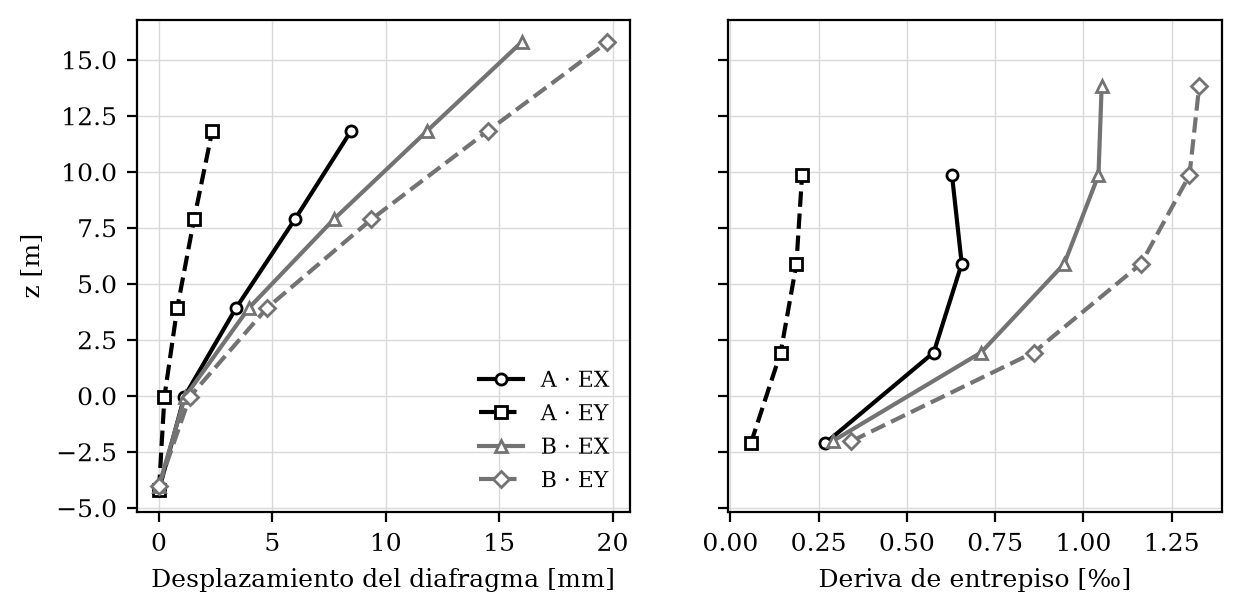
\includegraphics[width=0.92\textwidth]{final_derivas.png}
\caption{Desplazamiento del diafragma y deriva de entrepiso bajo EX y EY.}
\end{figure}

\begin{itemize}
  \item En A, la deriva máxima es 0,66~‰ (EX, piso 3) y 0,20~‰ (EY). En Y el
        edificio es mucho más rígido gracias a los muros largos de los ejes E
        e I.
  \item En B, la deriva máxima es 1,05~‰ (EX) y 1,33~‰ (EY), en los dos pisos
        superiores.
  \item \textbf{Torsión}: la rotación del techo de B es
        $r_z = 6{,}94\cdot10^{-4}$~rad bajo EX, unas \textbf{69 veces} la de A
        ($1{,}01\cdot10^{-5}$), y unas 14 veces bajo EY. La causa es la
        distribución excéntrica de muros y masa en B: núcleo al sur y un bloque
        superior sin núcleo.
  \item Todas las derivas están muy por debajo de los límites usuales (2~‰ en
        la NCh433), pero hay que recordar que $\alpha = 0{,}10$ es un valor
        fijo del enunciado, no un espectro de diseño.
\end{itemize}

% =====================================================================
\section{Superposición}

En un análisis \textbf{lineal elástico} la matriz de rigidez $K$ no depende de
la carga. Por eso la respuesta a una combinación es la suma ponderada de las
respuestas a cada caso:
\[
R\Big(\sum_i \lambda_i F_i\Big) = \sum_i \lambda_i R(F_i),
\]
donde $\lambda_i$ es el factor de cada caso. Por ejemplo, $\lambda_G = \lambda_Q = 1$
en GQ, y 1,2 y 1,6 en una combinación mayorada. La igualdad deja de valer si hay
no linealidad del material o geométrica (P--$\Delta$), porque entonces $K$
cambia con la carga. Se verificó numéricamente comparando una \textbf{corrida
directa} del caso combinado con la \textbf{suma} de los casos simples.

\begin{table}[h]
\centering
\caption{Verificación de la superposición: corrida directa contra suma de casos.}
\begin{tabular}{llrr}
\toprule
Edificio & Combinación & máx.\ $|\Delta R|$ [kN] & máx.\ $|\Delta u|$ [m] \\
\midrule
A & G+Q $\equiv$ GQ & $7{,}3\cdot10^{-12}$ & $7{,}6\cdot10^{-19}$ \\
A & G+EX & $6{,}2\cdot10^{-12}$ & $1{,}6\cdot10^{-17}$ \\
A & G+Q+EX & $3{,}6\cdot10^{-11}$ & $6{,}5\cdot10^{-18}$ \\
B & G+Q $\equiv$ GQ & $2{,}9\cdot10^{-11}$ & $8{,}7\cdot10^{-18}$ \\
B & G+EX & $5{,}6\cdot10^{-11}$ & $1{,}8\cdot10^{-16}$ \\
B & G+Q+EX & $6{,}0\cdot10^{-11}$ & $1{,}7\cdot10^{-16}$ \\
\bottomrule
\end{tabular}
\end{table}

A nivel de elemento también se comparó, componente por componente, la suma G+Q
con GQ. En A (112 elementos) la máxima diferencia es
$\Delta P = 3{,}9\cdot10^{-11}$~kN y $\Delta M = 1{,}9\cdot10^{-11}$~kN$\cdot$m.
En B (100 elementos) es $\Delta P = 4{,}7\cdot10^{-11}$~kN y
$\Delta M = 7{,}8\cdot10^{-10}$~kN$\cdot$m. El módulo
$M = \sqrt{M_y^2 + M_z^2}$ \emph{no} se superpone, porque no es lineal; por eso
la comparación se hace por componente. Las diferencias son del orden del error
de redondeo de un número de doble precisión.

\textbf{En el visor.} La verificación llega a Unity como dato: el contrato trae
el bloque \texttt{secciones.superposicion} con las tres combinaciones, y la
ventana P--M muestra el indicador $|\Delta P|$. El \emph{toggle} interactivo para
superponer casos con factores $\lambda$ \textbf{no se implementó}
(sección~\ref{sec:limitaciones}).

% =====================================================================
\section{Análisis global y verificaciones}

\begin{table}[h]
\centering
\caption{Verificaciones del análisis global (todas automáticas en la suite de tests).}
\begin{tabularx}{\textwidth}{lX}
\toprule
Verificación & Resultado \\
\midrule
Equilibrio global, 5 casos &
$|\Sigma F + \Sigma R| \le 1{,}1\cdot10^{-9}$~kN en A y $\le 3{,}5\cdot10^{-9}$~kN en B, en las tres componentes. \\
Conservación tributaria &
Carga de losa transferida $=$ $q\cdot A$ (error $3{,}6\cdot10^{-12}$~kN en A). \\
Corte basal &
$\Sigma R_x = -V$ y $\Sigma R_y = -V$ en EX y EY (A: 4\,541,74; B: 4\,817,11~kN). \\
Cierre de diagramas &
En las 238 vigas de A y las 215 de B, y en los 5 casos, los diagramas
evaluados en $x = L$ reproducen los esfuerzos del extremo $j$
(\texttt{localForce}). \\
Test analítico &
Viga biapoyada con carga central: la flecha de OpenSees coincide con
$PL^3/48EI$ (Euler--Bernoulli) a $< 10^{-10}$. \\
Contrato JSON &
Los tags apuntan a nodos existentes, la conectividad, los apoyos y la cobertura
de esfuerzos por caso están verificados (\texttt{test\_json\_contrato.py},
\texttt{test\_complejo.py}). \\
Reproducibilidad &
\texttt{python src/complejo.py --sin-visualizar} con openseespy 3.8.0.0, en un
entorno nuevo, seguido de \texttt{exportar\_ar.py --tags}, regeneró los
archivos de resultados con el mismo contenido (solo puede cambiar el fin de
línea). \\
\bottomrule
\end{tabularx}
\end{table}

\textbf{Corrección del signo de $M_z(x)$ (semana 6).} El visor evaluaba
$M_z(x) = M_z + V_y x + W_y x^2/2$. Lo correcto es
$M_z(x) = M_z - V_y x - W_y x^2/2$, porque en los ejes locales de OpenSees
$dM_z/dx = -V_y$. La evidencia fue la cabeza de la columna 14 en GQ: el visor
mostraba $-672{,}3$~kN$\cdot$m y OpenSees daba $+219$. Se corrigió en las tres
fórmulas del visor y en \texttt{src/secciones/diagramas.py}, y se agregó un test
que exige el cierre $M_z(L) = -M_{z,j}$.

% =====================================================================
\section{Fiber Sections}

El motor (\texttt{src/secciones/}) representa cada sección como un conjunto de
fibras:
\begin{itemize}
  \item \textbf{Hormigón}: \texttt{Concrete01} (Hognestad, sin tracción) con
        $\varepsilon_{c0} = -0{,}002$ y $\varepsilon_{cu} = -0{,}004$.
  \item \textbf{Acero de refuerzo}: \texttt{Steel01} con $f_y = 420$~MPa,
        $E_s = 200$~GPa y endurecimiento $b = 0{,}01$.
  \item \textbf{Discretización}: una grilla de $6\times6$, $12\times12$ o
        $20\times20$ fibras de hormigón, con la fibra al centro de cada celda, y
        \emph{una fibra por barra} con el área de esa barra.
\end{itemize}

\textbf{Por qué fibras explícitas.} En openseespy 3.8.0 el comando
\texttt{patch('rect')} dio un $EA$ un 93~\% mayor que el teórico en una celda
de $1\times1$. Con fibras explícitas, $EA$ y $EI$ coinciden con los valores
analíticos a $< 10^{-4}$. Un integrador 100~\% Python
(\texttt{analitica.py}) sirve de contraste independiente.

\begin{table}[h]
\centering
\caption{Secciones del catálogo y supuestos de armado.}
\begin{tabularx}{\textwidth}{lX}
\toprule
Sección & Armado y material \\
\midrule
Columna 0,70$\times$0,70 &
8$\phi$28, 4 por cara, recubrimiento al eje de 5~cm (plano 101, capa
RLE-PILAR). $\rho = 1{,}0$~\%. \\
Muros de A (5 secciones) &
\textbf{Supuesto}: los planos de A no traen la armadura de los muros (lo
confirmamos con otros grupos). Se usó doble malla $\phi$10@0,20 ($\rho_v \approx 0{,}003$)
y 6$\phi$16 por extremo en $L_b = \max(2t; 0{,}15L)$, con recubrimiento de 3~cm. \\
Muros de B (11 secciones) &
Bordes de 0,40~m con 4$\phi$16 y alma $\phi$12@0,20 por cara, con recubrimiento
de 5~cm (receta uniforme \texttt{muro\_b1}). \\
P.M.~300$\times$300$\times$20 (acero) &
Plastificación total del cajón. Acero A270ES, $f_y = 270$~MPa
(\textbf{supuesto}: los planos no indican la calidad). \\
\midrule
$f'_c$ de sección &
A: 30~MPa (G35); B: 25~MPa (valor representativo del enunciado). Los modelos
elásticos usan el $E$ de la sección~2. \\
\bottomrule
\end{tabularx}
\end{table}

% =====================================================================
\section{M--φ}

\textbf{Procedimiento} (\texttt{curva.py}). Sección en un elemento
\texttt{zeroLengthSection}. Primero se aplica la carga axial con
\texttt{LoadControl}; si no converge, se refina el paso en 1/2/4/8. Después,
con la carga axial fija, se aplica un momento unitario con
\texttt{DisplacementControl} sobre el giro. Se lee $M$ =
\texttt{getTime()} y $\varphi$ = \texttt{nodeDisp(2,3)}. La curva termina por
aplastamiento ($\varepsilon_c \le \varepsilon_{cu}$), por rotura del acero
($\varepsilon_{su} = 0{,}09$), por ablandamiento ($M < 0{,}85\,M_{max}$) o por
falta de convergencia.

\begin{figure}[h]
\centering
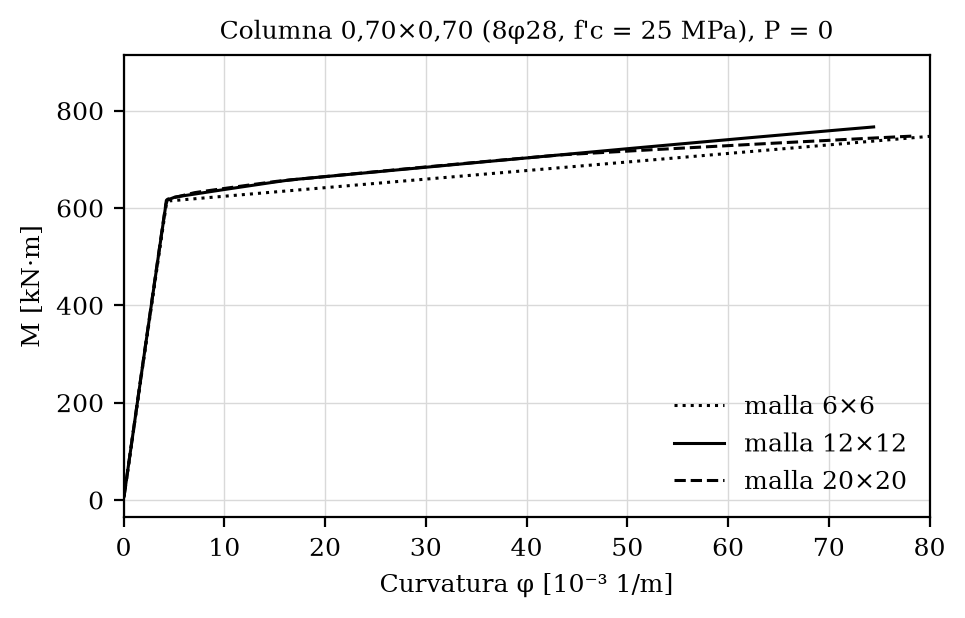
\includegraphics[width=0.7\textwidth]{final_mphi_columna.png}
\caption{Momento--curvatura de la columna 0,70$\times$0,70 con tres mallas.}
\end{figure}

\begin{table}[h]
\centering
\caption{Resultados M--φ de la columna ($P = 0$) y sensibilidad a la malla.}
\begin{tabular}{lrrl}
\toprule
Malla & $EI_0$ [kN$\cdot$m$^2$] & $M_{max}$ [kN$\cdot$m] & Fin de curva \\
\midrule
$6\times6$ & 144\,124 & 870 & tope de pasos \\
$12\times12$ & 145\,879 & 766 & no convergencia \\
$20\times20$ & 146\,399 & 748 & aplastamiento \\
Integrador analítico & 146\,991 & --- & --- \\
\bottomrule
\end{tabular}
\end{table}

\begin{itemize}
  \item La rigidez inicial agrietada con malla $12\times12$ difiere del valor
        analítico en $-0{,}8$~\%. Las tres mallas quedan dentro del 2~\% en
        $EI_0$.
  \item $EI_0 \approx 0{,}29\,E I_g$ (con $E = 2f'_c/\varepsilon_{c0} = 25$~GPa
        e $I_g = 0{,}020$~m$^4$). Este número justifica, por ejemplo, usar una
        inercia reducida en un análisis con secciones agrietadas.
  \item La fluencia aparece cerca de $M_y \approx 615$~kN$\cdot$m. $M_{max}$
        depende de dónde termina la curva, por eso cambia más con la malla que
        $EI_0$.
  \item Con $P = 3\,000$~kN: $EI_0 = 4{,}55\cdot10^5$~kN$\cdot$m$^2$ y
        $M_{max} = 1\,376$~kN$\cdot$m. La compresión retrasa el agrietamiento.
\end{itemize}

% =====================================================================
\section{P--M columna y muro}

\textbf{Barrido} (\texttt{pm.py}). Se calculan 17 niveles de carga axial, desde
la tracción pura ($-1{,}03\,f_y A_s$) hasta la compresión ($\approx 1{,}03\,P_0$).
Para cada nivel se obtiene la curva M--φ y se toma su momento máximo. El punto
balanceado corresponde a $\varepsilon_c = \varepsilon_{cu}$ en la fibra extrema y
$\varepsilon_s = \varepsilon_y$ en el acero opuesto. Convención: $P>0$ es
compresión.

\textbf{Verificación con cálculo a mano} (columna, $f'_c = 25$~MPa):
\begin{itemize}
  \item $P_{0,ACI} = 0{,}85 f'_c (A_g - A_s) + f_y A_s
        = 0{,}85\cdot25\,000\cdot0{,}48507 + 420\,000\cdot0{,}004926 = 12\,376{,}7$~kN,
        igual al motor.
  \item $P_{0,fibra} = f'_c(A_g-A_s) + E_s|\varepsilon_{c0}|A_s = 14\,097{,}3$~kN,
        también igual. La razón $P_{0,fibra}/P_{0,ACI} \approx 1{,}15$ se repite
        en las 12 secciones y viene de usar $f'_c$ en vez del bloque
        $0{,}85f'_c$. Es una diferencia de convención, no un error.
  \item El pico de la envolvente (4\,379~kN; 1\,530~kN$\cdot$m) se compara con
        el valor de aceptación del enunciado (4\,500; 1\,395): $-2{,}7$~\% en $P$
        y $+9{,}7$~\% en $M$, dentro de la tolerancia del 10~\%.
  \item Pilar de acero: $P_0 = f_y A = 6\,048$~kN y
        $M_p = f_y Z = 636{,}1$~kN$\cdot$m. Se verificó un punto con el eje
        neutro en las almas: $P = 756$~kN da $M = 622{,}9$~kN$\cdot$m, igual
        al cálculo analítico.
\end{itemize}

\begin{figure}[h]
\centering
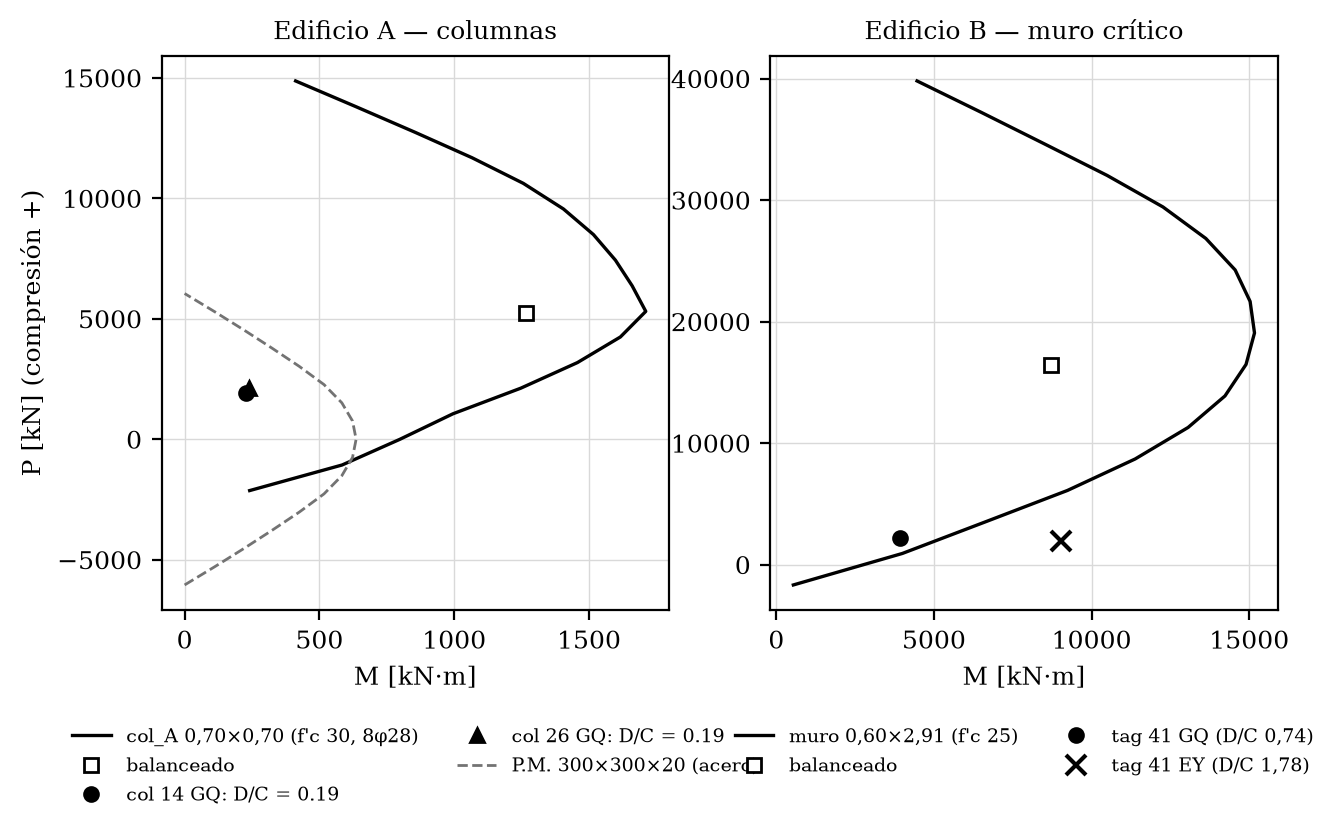
\includegraphics[width=\textwidth]{final_pm.png}
\caption{Diagramas de interacción con puntos de demanda. Izquierda: columna
de A con las columnas 14 y 26 de la app AR, y el pilar de acero. Derecha: muro
crítico de B (tag 41) en GQ y en EY.}
\end{figure}

\begin{table}[h]
\centering
\caption{Puntos característicos de las envolventes principales.}
\begin{tabular}{lrrrr}
\toprule
Sección & $A_s$ [cm$^2$] & $P_{0,ACI}$ [kN] & Balanceado $(P; M)$ & Pico $(P; M)$ \\
\midrule
col\_A 0,70$\times$0,70 ($f'_c$ 30) & 49,3 & 14\,438 & (5\,242; 1\,265) & (5\,308; 1\,711) \\
col 0,70$\times$0,70 ($f'_c$ 25) & 49,3 & 12\,377 & (4\,370; 1\,158) & (4\,379; 1\,530) \\
muro 0,60$\times$2,91 (B) & 38,7 & 38\,646 & (16\,407; 8\,705) & (19\,065; 15\,167) \\
muro\_A 0,20$\times$6,60 & 60,3 & 36\,037 & (15\,498; 19\,322) & (17\,256; 32\,551) \\
muro\_A 0,20$\times$7,25 & 63,4 & 39\,476 & (17\,066; 22\,942) & (18\,959; 39\,149) \\
P.M.~300$\times$300$\times$20 & 224 (acero) & 6\,048 & --- & (0; 636) \\
\bottomrule
\end{tabular}
\end{table}

\textbf{Error detectado en la revisión final.} Cinco envolventes de muros
largos tienen puntos con $M = 0$:
\begin{itemize}
  \item de A: muro\_A 0,30$\times$7,25 y 0,30$\times$8,90;
  \item de B: 0,20$\times$9,44, 0,20$\times$11,59 y 0,25$\times$7,95.
\end{itemize}
En esos niveles de $P$ la curva M--φ no converge y el barrido devuelve 0 en
lugar de descartar el punto. Las columnas y el muro 0,60$\times$2,91 no tienen
este problema. Las consecuencias están en la sección~\ref{sec:dc}.

% =====================================================================
\section{Demanda--capacidad}\label{sec:dc}

Para cada columna y muro, y para cada caso:
\[
\text{D/C} = \frac{M_d}{M_{cap}(P_d)}, \qquad M_d = \sqrt{M_y^2 + M_z^2},
\]
donde $M_{cap}(P_d)$ se interpola linealmente en la envolvente P--M de la
sección de ese \texttt{elementTag}, al mismo nivel de carga axial. La demanda se
evalúa en los dos extremos del elemento y gobierna el de mayor momento. En una
columna sin carga transversal $N$ es constante y $M$ varía linealmente, así que
el máximo siempre está en un extremo. Son demandas \textbf{de servicio}: no
tienen factores de mayoración y la capacidad no tiene factores $\phi$.

\begin{table}[h]
\centering
\caption{Demanda--capacidad de los elementos de referencia.}
\begin{tabular}{llrrrr}
\toprule
Elemento & Caso & $P_d$ [kN] & $M_d$ [kN$\cdot$m] & $M_{cap}$ [kN$\cdot$m] & D/C \\
\midrule
A col 14 (app AR) & GQ & 1\,899,9 & 229,5 & 1\,195,0 & 0,19 \\
A col 26 (app AR) & GQ & 2\,130,6 & 239,5 & 1\,249,2 & 0,19 \\
A pilar P.M.\ 73 & GQ & 3,8 & 215,0 & 636,1 & 0,34 \\
B col 2 & GQ & 8\,145,9 & 1\,278,4 & 1\,223,5 & \textbf{1,04} \\
B col 5 & GQ & 1\,773,4 & 1\,291,9 & 1\,143,1 & \textbf{1,13} \\
B muro 41 (0,60$\times$2,91) & GQ & 2\,175,2 & 3\,912,3 & 5\,270,9 & 0,74 \\
B muro 41 (0,60$\times$2,91) & EY & 1\,973,5 & 9\,022,8 & 5\,066,6 & \textbf{1,78} \\
\bottomrule
\end{tabular}
\end{table}

\begin{itemize}
  \item \textbf{Edificio A, columnas} (80, incluidos los 8 pilares de acero):
        el D/C máximo es 0,45 en GQ y 0,43 en EX. Ninguna supera 1.
  \item \textbf{Edificio B, columnas} (40): dos superan 1 en GQ (tags 5 y 2).
  \item \textbf{Muros con envolvente válida}: en B superan 1 dos en GQ (tag 77,
        a tracción, 1,21; tag 46, 1,04) y seis en EX y en EY (máx.\ 4,7--4,8,
        muros 42 y 46, que trabajan a tracción). En A supera 1 un muro en EX
        (tag 100, 2,15).
  \item \textbf{Fuera de la envolvente}: algunos muros de B tienen una
        tracción mayor que la de tracción pura de su sección, y ahí no hay
        capacidad que interpolar ni D/C. Son el muro 76 en GQ, los muros 41, 51
        y 52 en EX y los muros 76 y 77 en EY. Hay que leerlos como muros que
        exceden su capacidad a tracción. No están en los conteos de arriba.
  \item Los casos EX y EY se evalúan \emph{solos}, sin la gravedad que los
        acompaña. Por eso varios muros quedan a tracción y fuera de la zona útil
        de la envolvente. Para un diseño habría que evaluar las combinaciones
        reglamentarias mayoradas, que no forman parte del alcance.
  \item \textbf{No confiables}: los 16 muros de A (tags 84--99) y los 15 de B
        cuyas secciones tienen puntos con $M = 0$. Por ejemplo, el muro 95 de A
        aparece con D/C = 3,05 en GQ porque su capacidad interpolada cae en uno
        de esos puntos. Esos valores no deben leerse como una falla.
\end{itemize}

% =====================================================================
\section{Unity como pre/postprocesador}

\textbf{Arquitectura.} Python $\to$ contrato JSON $\to$ Unity. El visor
(\texttt{unity/EdificioSolidoUnity}, Unity 2022.3.62f3) \textbf{no calcula
nada}: reconstruye la escena completa desde
\texttt{StreamingAssets/edificio\_completo.json} (\texttt{UnityStickModel.cs},
\texttt{ModeloComplejo.cs} y \texttt{OrbitCamera.cs}). La escena
\texttt{Main.unity} pesa unos 10~KB, porque no tiene geometría guardada. Al
principio había una escena de 64~MB con la geometría guardada en ella, que
quedaba desactualizada respecto del JSON y era la causa del ``modelo deforme''
que veíamos. Eso se corrigió.

\textbf{Preprocesador.} El botón \emph{Recargar JSON} vuelve a leer el contrato
sin cerrar el editor y reconstruye todas las capas. En Android, la carga busca
primero \texttt{Application.persistentDataPath}. Así, \textbf{los datos se
actualizan en el teléfono sin recompilar el APK}
(\texttt{scripts/subir\_json\_telefono.ps1} hace el \texttt{adb push} y lo
verifica). El panel muestra la fuente y la fecha del JSON cargado.

\textbf{Postprocesador.} Al hacer clic en una columna, viga o muro se abre un
panel con:
\begin{itemize}
  \item tag, tipo, sección, material (hormigón o acero), nodos, restricciones y
        ejes locales;
  \item los esfuerzos $N, V_y, V_z, T, M_y, M_z$ del caso activo, evaluados en
        la posición $x$ del deslizador;
  \item una ventana de diagramas 2D y una ventana P--M con la envolvente, el
        punto balanceado, la demanda, $M_{cap}(P_d)$ y el D/C.
\end{itemize}

\textbf{Trazabilidad} (ejemplo: muro B tag 41):
\begin{enumerate}
  \item \texttt{elementTag} 41 en OpenSees (nodos 49$\to$50);
  \item \texttt{esfuerzos\_completos.GQ."41"} y \texttt{metadatos."41"} en el JSON;
  \item el \texttt{BoxCollider} del panel del muro en Unity;
  \item el panel de consulta: $N = 2\,175{,}2$~kN y
        $M_z = 3\,909{,}2$~kN$\cdot$m en $x = 0$;
  \item la sección \texttt{muro0.60x2.91} del catálogo;
  \item $M_{cap} = 5\,270{,}9$~kN$\cdot$m, D/C = 0,74.
\end{enumerate}

\textbf{Vista combinada.} Desde la sesión 28, los dos edificios se dibujan lado
a lado. La cámara inicial queda de frente al eje J de A, con B a la izquierda, y
la sensibilidad de rotación subió de 0,25 a 3 (la ajustamos tras la revisión
del profesor). Solo cambian la cámara y el desplazamiento con que se dibujan los
edificios: las coordenadas de los datos no se tocan.

% =====================================================================
\section{Visualización de apoyos, cargas, ejes y diagramas}

\begin{table}[h]
\centering
\caption{Capas del visor y su estado.}
\begin{tabularx}{\textwidth}{llX}
\toprule
Capa & Estado & Qué muestra y de dónde sale \\
\midrule
Apoyos & completa & Zapatas o conos en los 23 + 20 apoyos empotrados (\texttt{apoyos}). \\
Cargas G / Q & completa & Cargas distribuidas por viga (\texttt{cargas.vigas[]}: $q_G$, $q_Q$). \\
Cargas sismo & completa & Flechas $F_i$ por nivel para EX/EY (\texttt{cargas.sismo}). \\
Tributaria 45\textdegree & parcial & Mosaico de reparto por viga; dibuja solo $q_G$. \\
Ejes locales & parcial & Están en \texttt{metadatos.ejes\_locales} y orientan los diagramas, pero no se dibujan como triadas. \\
Deformada & completa & Casos Base/G/GQ/EX/EY con amplificación 0--2000 (desplazamientos de los nodos maestros). \\
Diagramas 3D & completa & $N$, $M_y$ y $M_z$ sobre cada elemento, con escala automática. \\
Ventana 2D & completa & Axial, corte ($V_z$, $V_y$) y momento ($M_y$, $M_z$) con los extremos, el máximo y su posición. $T$ solo se muestra como valor numérico. \\
Material & completa & Los elementos de acero se dibujan con el lado de su perfil (0,30~m) y un material metálico gris. \\
\bottomrule
\end{tabularx}
\end{table}

Los diagramas 3D se escalan para que su amplitud mida $\approx 15$~\% de la
luz. Por eso sirven para ver la forma; los valores exactos se leen en el panel y
en la ventana 2D.

% =====================================================================
\section{Modificación del modelo}

\textbf{Flujo}: editar un dato $\to$ volver a analizar $\to$ refrescar las
cachés de secciones $\to$ exportar el contrato $\to$ \emph{Recargar JSON}. Los
cuatro primeros pasos son comandos documentados en el README; el último es un
botón. No hace falta editar ninguna escena a mano.

\begin{table}[h]
\centering
\caption{Modificaciones ejecutadas de punta a punta, con el antes y el después.}
\begin{tabularx}{\textwidth}{Xll}
\toprule
Modificación & Antes & Después \\
\midrule
\textbf{MOD1} B: sobrecarga \texttt{SC\_PISO} 3,0 $\to$ 4,0~kN/m$^2$ & Q = 11\,029,6~kN & Q = 14\,423,3~kN \\
\quad muro 41, GQ & D/C = 0,74 & D/C = 0,79 \\
\textbf{MOD2} B: espesor del muro \texttt{MUROS\_V[0]} 0,60 $\to$ 0,70~m & $P_{0,ACI}$ = 38\,646~kN & 44\,830~kN \\
\quad techo EX / EY & 16,00 / 19,77~mm & 15,74 / 19,28~mm \\
\textbf{MOD3} A: viga secundaria F--G (niveles 1 y 2) y pilar metálico 349 & 343 elementos, G = 45\,236,5 & 354, G = 45\,417,4 \\
\quad viga 134 (GQ): $M_i$ / $M_j$ & $-114{,}3$ / $-159{,}6$~kN$\cdot$m & $-220{,}0$ / $-265{,}3$~kN$\cdot$m \\
\textbf{MOD4} A: pilares y diagonales de acero (material, perfil y P--M propia) & curva de hormigón & curva P.M.\ de acero \\
\bottomrule
\end{tabularx}
\end{table}

\begin{itemize}
  \item MOD1 y MOD2 se ejecutaron y después se volvió al estado canónico.
  \item MOD3 y MOD4 son cambios permanentes, hechos al revisar los planos.
  \item Al cambiar la sección, la envolvente creció más que la demanda. Con más
        carga de uso, la demanda crece y la capacidad casi no cambia.
  \item Cambiar la inercia ($EI$) modifica la \emph{demanda}: desplazamientos,
        derivas y reparto de momentos en una estructura hiperestática. Cambiar la
        cuantía modifica la \emph{capacidad}, es decir la curva P--M, pero no los
        esfuerzos del análisis elástico.
\end{itemize}

% =====================================================================
\section{AR}

\subsection{Objetivo y flujo}

La app Android (\texttt{Assets/Scenes/AR\_Inspeccion.unity}, AR Foundation 4.2.0
con ARCore) es una herramienta de inspección en obra. El usuario elige un
elemento de una lista de \textbf{nueve} (caso GQ, Edificio A), marca su
posición real con el teléfono y ve encima sus diagramas $N$, $V$ y $M$; en
columnas y muros también ve el panel P--M. Los elementos son:
\begin{itemize}
  \item columnas \textbf{14} y \textbf{26} (ejes F y G, A3);
  \item vigas \textbf{134} y \textbf{350} (F--G, A3) y \textbf{354} (la viga
        secundaria F--G);
  \item los elementos de acero del voladizo del eje F: la viga \textbf{337}, el
        pilar \textbf{340} y la diagonal \textbf{342};
  \item el muro \textbf{105}.
\end{itemize} \textbf{No se usa marcador
impreso}: la referencia es el propio elemento.

\begin{center}
elemento real $\to$ pose ARCore $\to$ \texttt{ARAnchor} $\to$ transformación
$\to$ geometría del elemento $\to$ resultado
\end{center}

Los valores no se calculan en el teléfono. Son los muestreos de
\texttt{ar\_elementos.json}, que \texttt{src/ar/exportar\_ar.py} exporta desde
los mismos resultados verificados. Hay 17 tests que comparan esos diagramas con
\texttt{localForce} de OpenSees en los dos extremos.

\subsection{Transformación}

\[
\mathbf{p}_{mundo} = \mathbf{t}_A + \Delta h\,\hat{\mathbf{y}} +
R_y(\theta)\,\big(C\,\mathbf{p} - \mathbf{a}\big), \qquad
C = \begin{bmatrix}1&0&0\\0&0&1\\0&1&0\end{bmatrix}
\]

\begin{itemize}
  \item $C$ pasa de OpenSees $(x,y,z)$ a Unity $(x,z,y)$, con
        $\det C = -1$: cambia de un sistema de mano derecha a uno de mano
        izquierda, así que la geometría no sale espejada.
  \item $\mathbf{a}$ es el punto de anclaje del elemento: su base, a nivel del
        piso.
  \item $R_y(\theta)$ es solo un giro en planta. La vertical la fija la gravedad
        que mide ARCore.
  \item $\Delta h$ es el ajuste de piso, en pasos de $\pm5$~cm.
  \item $\mathbf{t}_A$ es la posición del ancla. La escala es 1:1.
  \item En una viga, $\theta$ sale de la dirección entre los dos apoyos
        marcados y el ancla queda en el punto medio. La app avisa si la
        distancia medida difiere de $L$ en más de un 10~\%.
\end{itemize}

\subsection{Modos de colocación (versión final: corrección 10 + cambio\_01)}

\begin{itemize}
  \item \textbf{Encuadrar: 4 esquinas.} Se tocan las cuatro esquinas de la cara
        del elemento, en cualquier orden. La primera esquina fija la distancia y
        las otras tres se proyectan sobre un plano de frente a la cámara, así
        que el diagrama queda como una figura 2D, igual que una imagen impresa.
        Se dibuja dentro de ese recuadro, en 3 bandas ($N$, $V$ y $M$), sin
        anillo y sin profundidad. Los rótulos quedan impresos en ese plano y
        con el tamaño justo para caber.
  \item \textbf{Marcar base (anillo).} Se toca el pie de la columna. El punto se
        lleva media sección hacia adentro, hasta el eje.
  \item \textbf{Marcar viga: apuntar a ella.} Se apunta a la cara inferior de la
        viga cerca de cada columna, usando la profundidad de ARCore. El eje de
        la viga queda sobre los ejes de las columnas.
  \item \textbf{Marcar viga: pie de columnas}, la alternativa al modo anterior.
  \item Además: \emph{Panel 2D} con los mismos valores en un recuadro fijo,
        siempre legible; \emph{Piso $\pm$5~cm}; \emph{Quitar ancla};
        \emph{Diag}, con un diagnóstico de tracking y profundidad; y un menú
        plegable.
  \item Desde cambio\_01, todos los rótulos (también los del dibujo 1:1)
        \textbf{quedan fijos al colocarse}: ya no giran ni cambian de tamaño
        cuando la cámara se mueve.
\end{itemize}

Cada elemento tiene su propia ancla. Si ARCore pierde el seguimiento, los
diagramas se ocultan en vez de quedar flotando en un lugar equivocado.

\subsection{Precisión y resultados}

\begin{figure}[h]
\centering
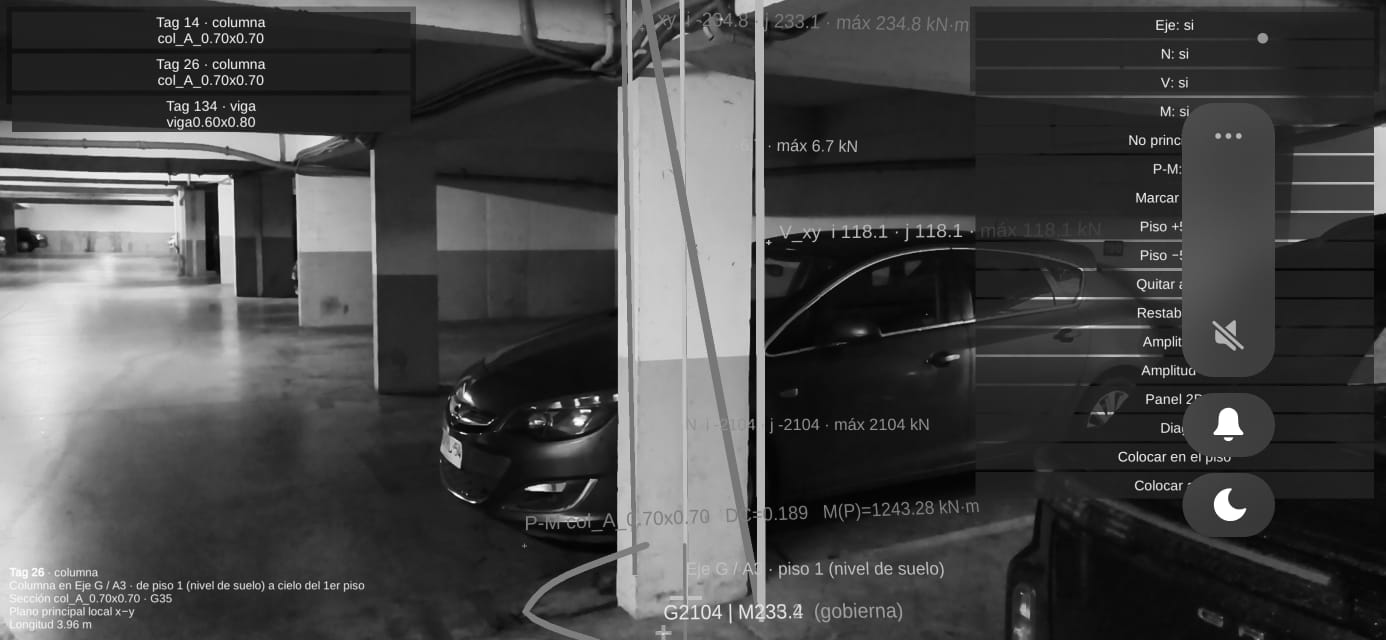
\includegraphics[width=0.49\textwidth]{final_ar_columna26.png}\hfill
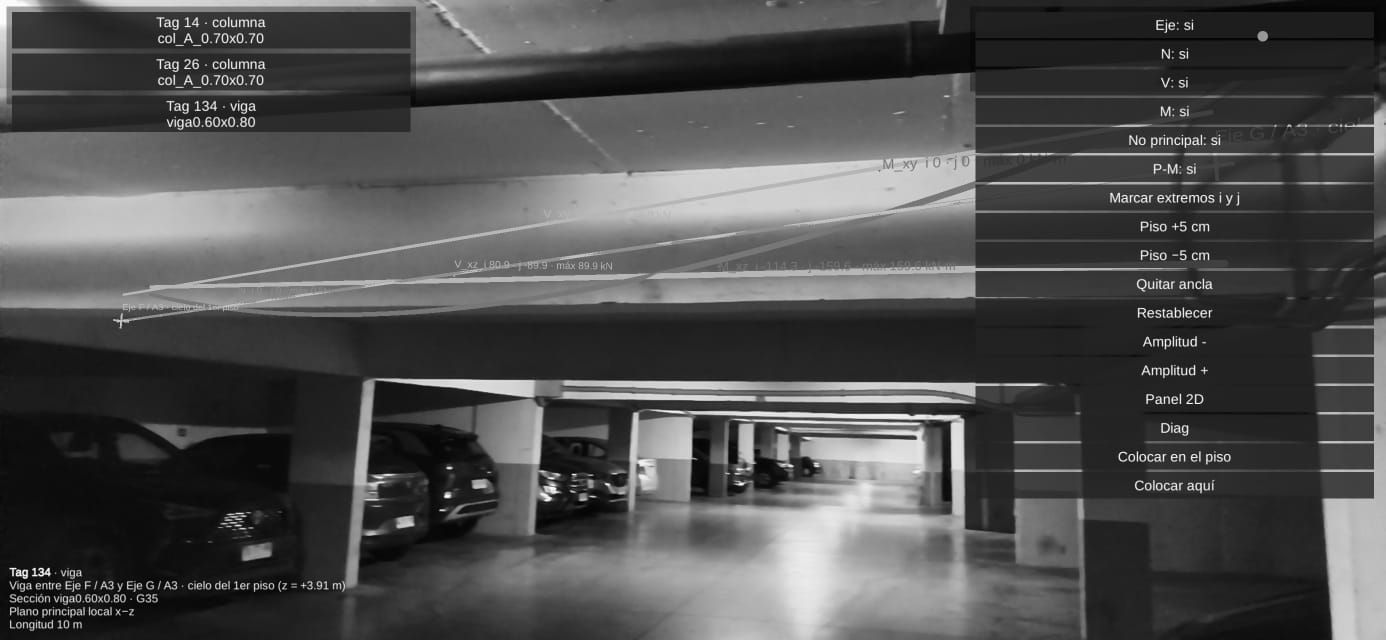
\includegraphics[width=0.49\textwidth]{final_ar_viga134.png}
\caption{Prueba de terreno de la semana 6: columna 26 (izquierda) y viga 134
(derecha). Los rótulos de las fotos son anteriores a las sesiones 26--29; los
valores vigentes están en la tabla siguiente.}
\end{figure}

\begin{itemize}
  \item \textbf{Alineamiento medido} sobre la foto de la columna 26, con escala
        de 6~mm/px: el error lateral es de \textbf{1--2~cm} en el pie y en la
        cabeza, sin inclinación apreciable.
  \item \textbf{Presupuesto de error esperado}: 2--5~cm. Contribuyen el toque
        ($\pm$2--5~cm), el piso ($\pm$5~cm, corregible), la verticalidad
        (0,2--0,5\textdegree) y la deriva de ARCore (1--2~\% de lo caminado).
  \item Esa precisión alcanza para identificar el elemento, la cara y el
        extremo $i/j$, pero no para medir deformaciones, que son milimétricas.
\end{itemize}

\begin{table}[h]
\centering
\caption{Valores vigentes de los elementos AR (caso GQ, \texttt{ar\_elementos.json}).}
\small
\begin{tabular}{llrrrr}
\toprule
Tag & Elemento (sección) & $N$ [kN] & $M_i$ [kN$\cdot$m] & $M_j$ [kN$\cdot$m] & D/C \\
\midrule
14 & Columna F/A3 (0,70$\times$0,70) & $-1\,899{,}9$ & $-223{,}1$ & 217,0 & 0,19 \\
26 & Columna G/A3 (0,70$\times$0,70) & $-2\,130{,}6$ & $-231{,}4$ & 230,9 & 0,19 \\
134 & Viga F--G/A3, $L = 10$~m (V.60/80) & $\approx 0$ & $-220{,}0$ & $-265{,}3$ & --- \\
350 & Segundo tramo de la 134 (misma viga física) & $\approx 0$ & $-220{,}0$ & $-265{,}3$ & --- \\
354 & Viga secundaria F--G, $L = 7{,}25$~m ($M^+ = 139{,}2$) & $\approx 0$ & $-42{,}0$ & $-66{,}4$ & --- \\
337 & Viga de acero V.M.\ 300$\times$300$\times$5, $L = 7{,}5$~m & 0,1 & $-18{,}4$ & 14,3 & --- \\
340 & Pilar de acero P.M.\ 300$\times$300$\times$20 & $-12{,}1$ & $-10{,}5$ & 14,3 & 0,02 \\
342 & Diagonal de acero V.M.\ 300$\times$300$\times$5, $L = 5{,}85$~m & 23,9 & $-6{,}4$ & $-1{,}3$ & --- \\
105 & Muro M2a (0,20$\times$3,70) & $-219{,}8$ & 125,2 & 140,4 & 0,04 \\
\bottomrule
\end{tabular}
\end{table}

\begin{figure}[h]
\centering
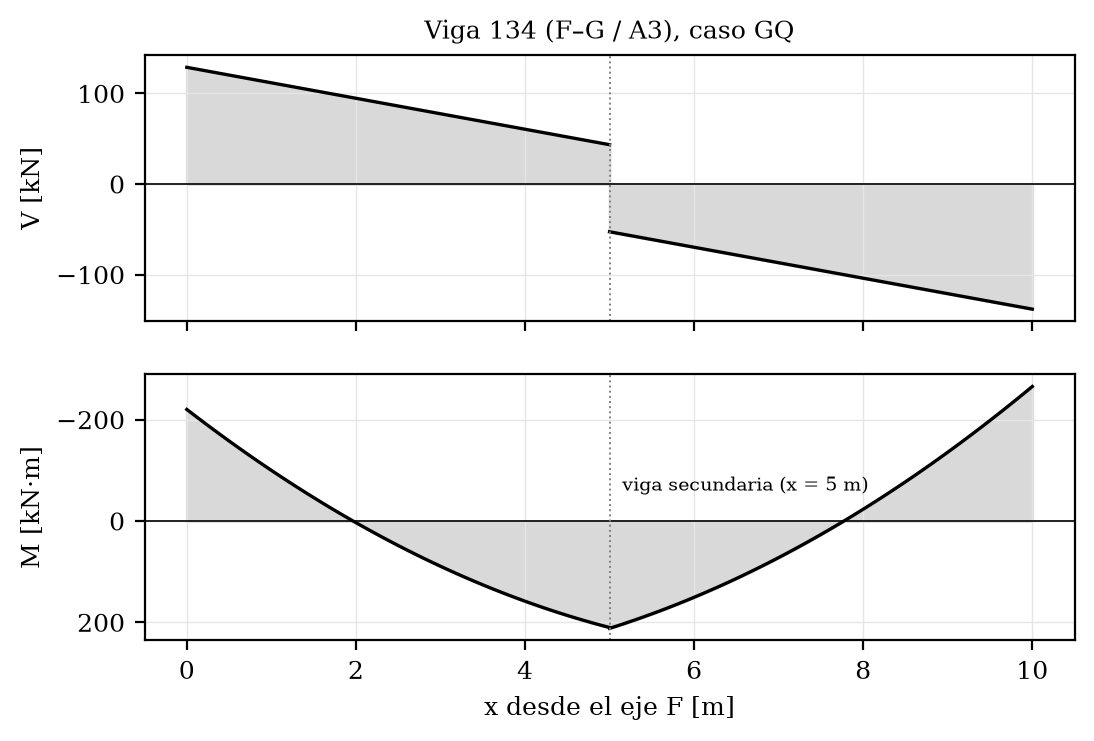
\includegraphics[width=0.72\textwidth]{final_viga134.png}
\caption{Viga 134 en GQ. La viga secundaria apoyada en $x = 5$~m introduce un
salto de corte de $\approx 96$~kN.}
\end{figure}

La viga 134 quedó partida en $x = 5$~m por la viga secundaria. La app la sigue
mostrando como \emph{una} viga física de columna a columna, porque encadena los
tramos 134 y 350. El momento al centro es $+211{,}9$~kN$\cdot$m. El
equilibrio se cumple: $(|M_i| + |M_j|)/2 + M_c \approx 454{,}6$~kN$\cdot$m,
contra $wL^2/8 + PL/4 = 453{,}8$~kN$\cdot$m. La diferencia, de 0,2~\%, es el
salto de $\approx 1{,}7$~kN$\cdot$m que produce en $x = 5$~m la torsión de la
viga secundaria.

La lista de la app se arma sola a partir del JSON, así que pasar de 3 a 9
elementos no requirió tocar la interfaz: bastó con regenerar el contrato
(\texttt{exportar\_ar.py --tags ...}). Hay dos detalles a tener en cuenta:
\begin{itemize}
  \item El tag 350 es el segundo tramo de la viga 134. Como el exportador
        encadena los tramos, se ve como la misma viga física.
  \item La diagonal 342 aparece con tipo ``viga'', porque en el modelo es
        \texttt{vigas\_y} y el exportador no tiene un tipo ``diagonal''.
\end{itemize}

\textbf{Build}: Android, minSdk 24, IL2CPP ARM64, OpenGLES3, ARCore requerido,
paquete \texttt{com.mcoc.edificiocomplejo.ar}. Se genera desde el menú
\emph{Tools/MCOC/Build Android AR}. El APK final
(\texttt{MCOC\_AR\_EdificioComplejo.apk}, 24,6~MB, con los 9 elementos) se
compiló en Windows con 153/153 tests de EditMode y 0 errores de compilación. Va
adjunto al Release \texttt{entrega-final}.

% =====================================================================
\section{Sidequests implementados}

\begin{itemize}
  \item \textbf{Sidequest ``carga móvil'': no implementada.} Quedó documentada,
        con el diseño para una versión 2 (línea de influencia, deslizador de
        posición y conservación $\Sigma P_i = W$), en el informe de la
        semana~5. El modelo es lineal y estático, y el edificio no tiene cargas
        vehiculares reglamentarias.
\end{itemize}

Extensiones que sí implementamos, fuera del núcleo pedido:
\begin{enumerate}
  \item \textbf{Datos actualizables en el teléfono sin recompilar}: precedencia
        \texttt{persistentDataPath} $\to$ \texttt{StreamingAssets}, script
        \texttt{adb} con verificación y botón \emph{Usar JSON del APK}.
  \item \textbf{Diagrama de interacción de pilares metálicos}: un perfil cajón
        con plastificación total, verificado analíticamente
        (\texttt{src/secciones/acero.py}).
  \item \textbf{App AR con nueve elementos} (hormigón y acero; columna, viga,
        diagonal y muro), sin cambiar la interfaz, porque la lista sale del
        contrato.
  \item \textbf{Cuatro modos de colocación AR y Panel 2D}, con la vertical
        corregida, el ajuste de piso y la ocultación al perder el tracking.
  \item \textbf{Complejo A+B en un solo visor}, con la fusión de contratos y la
        vista lado a lado.
  \item \textbf{Viga física encadenada} en la app AR: los tramos colineales
        unidos en nudos sin columna se muestran como una sola viga.
\end{enumerate}

% =====================================================================
\section{QA y tests}

\begin{table}[h]
\centering
\caption{Suite de Python: \texttt{python -m pytest tests -q} da 169 tests aprobados.}
\begin{tabularx}{\textwidth}{lrX}
\toprule
Archivo & Tests & Qué protege \\
\midrule
\texttt{test\_benchmark.py} & 38 & Geometría de A, secciones, conservación tributaria, equilibrio, superposición, Euler--Bernoulli y modelo base intacto (190/321). \\
\texttt{test\_secciones.py} & 40 & Motor de fibras, P--M, catálogos A y B, demandas, superposición y overlay del visor. \\
\texttt{test\_json\_contrato.py} & 22 & Contrato del visor: tags, nodos, conectividad y apoyos. \\
\texttt{test\_ar\_elementos.py} & 17 & Contrato AR, diagramas contra \texttt{localForce}, D/C y viga encadenada. \\
\texttt{test\_viga\_secundaria\_fg.py} & 9 & Viga secundaria: conteos, tags, diafragma, áreas tributarias y +87~kN por nivel. \\
\texttt{test\_esfuerzos\_a.py} & 8 & Diagramas de las 238 vigas de A: equilibrio y cierre. \\
\texttt{test\_complejo.py} & 8 & Fusión A+B y contrato unificado. \\
\texttt{test\_acero\_elementos.py} & 5 & Elementos de acero: material, perfil y P--M propia. \\
\texttt{test\_edificio\_b/} (5 archivos) & 22 & Geometría, análisis, sismo, tributario y esfuerzos de B. \\
\bottomrule
\end{tabularx}
\end{table}

\begin{itemize}
  \item \textbf{Unity}: Test Runner EditMode, \textbf{153/153}. Cubren la
        colocación, el encuadre, el piso, los rótulos, el panel 2D, la interfaz
        (que no haya botones tapados) y la configuración XR de Android.
  \item Para iterar sin abrir Unity, 150 de esos tests (todos menos los 3 de
        XR) se compilan con Mono contra \emph{stubs} de UnityEngine. El resultado
        se confirmó después en Unity.
  \item \textbf{Entornos probados}: Windows (equipo del grupo) y Linux.
        Python 3.11 y 3.12, con openseespy 3.7.1.2 y 3.8.0.0: los 169 tests
        pasan en todas esas combinaciones.
  \item \textbf{Pruebas de terreno}: las pruebas con el teléfono, con fotos y
        videos, guiaron las correcciones 3 a 10 de la app. El cambio\_01 (encuadre
        plano y rótulos fijos) y la lista de 9 elementos se verificaron con los
        tests (153/153) y con el APK compilado.
  \item \textbf{Regla de trabajo}: ningún cambio se aceptó con tests en rojo,
        y cada número de este informe sale de un archivo de \texttt{results/}
        regenerable.
\end{itemize}

% =====================================================================
\section{Limitaciones}\label{sec:limitaciones}

\begin{enumerate}
  \item \textbf{Modelo lineal elástico de primer orden}: no considera P--$\Delta$,
        agrietamiento ni plasticidad en el análisis global. Las inercias son
        brutas, aunque el M--φ indica $EI_{cr} \approx 0{,}3\,EI_g$.
  \item \textbf{Sismo}: método pseudoestático con $\alpha = 0{,}10$ fijo, sin
        análisis modal ni espectral, sin torsión accidental y sin combinaciones
        reglamentarias mayoradas.
  \item \textbf{Capacidad}: el D/C es de servicio. La flexión biaxial se
        combina como $\sqrt{M_y^2+M_z^2}$ contra una curva uniaxial. Las vigas
        no tienen armadura modelada (solo demanda) y no hay verificación de
        corte ni de pandeo.
  \item \textbf{Envolventes con $M = 0$} en cinco secciones de muros largos,
        por falta de convergencia (sección~\ref{sec:dc}). Los D/C de esos
        31 muros no son confiables. \emph{Corrección pendiente}: descartar o
        refinar los puntos que no convergen en \texttt{pm.py}.
  \item \textbf{Supuestos de armado y materiales}: la armadura de los muros de A
        no está en los planos; para el acero de los pilares se supuso A270ES; en
        las secciones de B se usó $f'_c = 25$~MPa.
  \item \textbf{Visor}: no tiene \emph{toggle} de superposición interactiva;
        los ejes locales no se dibujan; la capa tributaria muestra solo $q_G$;
        $T$ no tiene gráfico; el visor clásico no tiene gestos táctiles.
  \item \textbf{AR}: nueve elementos del Edificio A y un solo caso (GQ);
        colocación manual. \texttt{src/complejo.py} exporta por defecto solo
        3 elementos: para regenerar el contrato de 9 hay que correr
        \texttt{exportar\_ar.py --tags} (README, paso 3). La
        precisión es de centímetros. La viga 134 coincide con la realidad solo
        en el Edificio A. Las versiones intermedias (correcciones 8--9)
        empeoraron en terreno y hubo que volver atrás en parte.
  \item \textbf{Bug conocido}: \texttt{scripts/semana03\_run.py --recalcular}
        parte con la caché vacía y borra las curvas genéricas de B. Para
        refrescar solo las combinaciones hay que usar
        \texttt{superposicion.verificar} sobre la caché cargada.
\end{enumerate}

% =====================================================================
\section{Uso de IA}

\subsection{Herramientas}

\begin{itemize}
  \item \textbf{Claude} (Anthropic): en un proyecto de claude.ai con los planos
        y la bitácora como contexto, y en sesiones de agente con acceso a una
        copia del repositorio.
  \item \textbf{opencode}: un agente de código con acceso directo al
        repositorio en Windows, usado para integrar cambios en varios archivos,
        actualizar tests y compilar.
\end{itemize}

\subsection{Tareas delegadas}

\begin{itemize}
  \item Scripts de extracción DXF y fichas de geometría (que nosotros revisamos
        contra los planos dibujados).
  \item Módulos del modelo (\texttt{voladizos.py},
        \texttt{vigas\_secundarias.py}, \texttt{pilares\_metalicos.py}) y el
        modelo de B.
  \item El motor de secciones completo (\texttt{src/secciones/}, 13 módulos).
  \item El visor Unity y la app AR: unas 9\,200 líneas de C\# y 153 tests.
  \item Los tests de Python, la redacción inicial de los informes semanales y
        este informe, que nosotros revisamos.
\end{itemize}

\subsection{Errores detectados}

\begin{longtable}{p{0.45\textwidth}p{0.48\textwidth}}
\toprule
Error del agente o de la herramienta & Cómo se detectó y qué se hizo \\
\midrule
\endhead
Signo de $M_z(x)$ en el visor ($-672{,}3$ en lugar de $+219$~kN$\cdot$m). &
Comparando con \texttt{localForce} de OpenSees. Se corrigió la fórmula y se
agregó un test de cierre. \\
Los 20 muros de 0,20~m del bloque superior de B tomaban la sección de la columna. &
Revisión del catálogo; ahora hay un test que exige 60 muros con sección propia. \\
Las columnas no mostraban su P--M en el visor (clave de catálogo). &
Prueba en Play; se agregó un alias y una búsqueda en tres niveles. \\
Un verificador entregó $M(0) \approx 220$~kN$\cdot$m (no había llegado al pico). &
Contraste con el integrador analítico; el valor real es 750--870. \\
Los elementos de acero aparecían como hormigón y con la P--M de una columna de HA. &
Lo notamos en el visor; ahora tienen material, perfil y P--M de acero propios. \\
El agente cambió los finales de línea de un archivo completo al editar una línea. &
Lo vimos en el diff; se revirtió y se hizo una edición que conserva los bytes. \\
Las correcciones 8 y 9 de la app AR empeoraron la colocación en terreno (esquinas en el piso detrás del elemento, textos enormes). &
Con fotos y videos de las pruebas. En la corrección 10 se volvió en parte a la versión anterior y se fijó el tamaño de los textos. \\
Al consolidar la entrega en un segundo equipo, la sincronización automática
reemplazó la bitácora principal por la del equipo de compilación, y se perdió el
registro de las sesiones 22--29. &
Se detectó al comparar los dos paquetes de entrega. Se restauró
\texttt{docs/bitacora.md} y la otra quedó como
\texttt{docs/bitacora\_apk\_pablo.md}. \\
En el repo consolidado, un helper de \texttt{LlenarElementosTests.cs} recorría
el diccionario de elementos como si fuera una lista y no compilaba. Eso habría
dejado sin compilar el ensamblado Editor, con los tests y los menús de build. &
Se detectó compilando los tests fuera de Unity. Se corrigió usando
\texttt{Raiz().EnOrden()}; ahora pasan 150 de 150 sin Unity (153 con XR). El
APK no se vio afectado: se compiló desde una copia que sí estaba bien. \\
Un test de interfaz de Unity comparaba un botón consigo mismo. &
Falló en el Test Runner de Windows; se excluyó la comparación consigo mismo. \\
Envolventes P--M con puntos $M = 0$ (sin convergencia). &
Se detectó en la revisión de este informe; queda documentado como pendiente. \\
\bottomrule
\end{longtable}

\subsection{Verificaciones}

No aceptamos un número solo porque el agente lo afirmara. Cada resultado se
contrastó de al menos una de estas formas:
\begin{itemize}
  \item cálculo a mano: $P_0$, $M_n$ por par de fuerzas, $M_p$ del acero y
        $wL^2/8$;
  \item comparación con OpenSees: \texttt{localForce} y reacciones;
  \item equilibrio y conservación de carga;
  \item la suite de 169 + 153 tests;
  \item pruebas de terreno con el teléfono;
  \item la reproducción completa del pipeline en un entorno limpio.
\end{itemize}
El propio verificador también falló una vez ($M(0) \approx 220$). Por eso
exigimos una referencia independiente tanto para el agente como para el
verificador.

\subsection{Contribución real del agente}

Siendo honestos: \textbf{la mayor parte de las líneas de código las escribieron
los agentes}, tanto en Python como en C\#. Lo que aportamos nosotros fue:
\begin{itemize}
  \item las decisiones de alcance (qué elementos, qué niveles, qué supuestos);
  \item la lectura y validación de los planos;
  \item la definición de qué había que verificar y con qué referencia;
  \item las pruebas en el teléfono y en terreno;
  \item el criterio para rechazar versiones que empeoraban;
  \item la defensa técnica de los resultados.
\end{itemize}
Sin esa supervisión, varios errores de la tabla anterior habrían llegado a la
entrega.

% =====================================================================
\section{Contribución individual}

\begin{table}[H]
\centering
\caption{Contribución de cada integrante.}
\small
\begin{tabularx}{\textwidth}{p{2.4cm}XXXX}
\toprule
Integrante & Contribuciones & Módulo revisado & Error detectado & Concepto aprendido \\
\midrule
Nicolás Letelier &
Coordinación del trabajo con los agentes de IA;
cargas, sismo y verificaciones; motor de secciones; edición de los informes. &
\texttt{src/secciones/} (fibras, P--M, D/C) y \texttt{benchmark\_3d/cargas.py}. &
El signo de $M_z(x)$ en el visor: en la cabeza de la columna 14 mostraba $-672$
y OpenSees daba $+219$~kN$\cdot$m. &
La superposición solo vale con $K$ constante (análisis lineal). La inercia
cambia la demanda; la cuantía cambia la capacidad. \\
\midrule
Pablo Arancibia &
Implementación del modelo base del Edificio A en OpenSeesPy; compilación
de los APK en Windows (correcciones, cambio\_01 y versión final de 9
elementos); pruebas de terreno de la app AR. &
\texttt{benchmark\_3d/construir.py} y la app AR en el teléfono. &
En terreno: las esquinas del encuadre caían en el piso detrás del elemento
(corrección 8). &
Cómo el diafragma rígido reparte la carga sísmica, y el cambio de ejes
OpenSees $\to$ Unity $\to$ ARCore. \\
\midrule
Oscar Rodríguez &
\textbf{Arquitectura}: trabajo con los planos DXF y diseño de los dos
edificios para el modelo; repositorio y entregas en GitHub; visor Unity y
presentación de la parte de AR. &
Visor Unity: \texttt{Unity\-Stick\-Model.cs} y \texttt{OrbitCamera.cs}. &
La escena de 64~MB con la geometría guardada en ella, que mostraba un modelo
deforme distinto del JSON. &
Separar datos y diseño en el APK: el JSON se actualiza sin recompilar. \\
\bottomrule
\end{tabularx}
\end{table}

% =====================================================================
\section{Honors Track}

El grupo declara dos de los cinco ítems Honors (H1--H5) y explica por qué no
aplican los demás:

\begin{table}[H]
\centering
\caption{Declaración Honors Track.}
\small
\begin{tabularx}{\textwidth}{lcX}
\toprule
Ítem & ¿Aplica? & Justificación \\
\midrule
H3 --- AR estructural avanzada & Sí &
La app coloca elementos reales a escala 1:1 marcando el propio elemento, sin
marcador impreso. Dibuja $N$, $V$ y $M$ y muestra el panel P--M con el D/C junto
al elemento. Tiene nueve elementos, un ancla de ARCore por elemento, encuadre
plano y una precisión medida de 1--2~cm (sección~16). \\
H5 --- Capacidad / análisis avanzado & Sí &
Análisis no lineal de sección por fibras: M--φ, envolventes P--M y D/C por
elemento contra la envolvente de su sección. Incluye la P--M de los pilares de
acero, la superposición verificada y las capacidades regeneradas al modificar
el modelo (secciones 9 a 12 y 15). No incluye P--M biaxial ni segundo orden. \\
H1 --- VR (Cardboard) & No & No se desarrolló. \\
H2 --- AR multimarcador / persistencia & No & Marcado a toque, con un ancla por elemento y sin imágenes aumentadas. \\
H4 --- Reanálisis en vivo & No & El análisis corre en el PC; el teléfono recibe datos (\emph{Recargar JSON} o \texttt{adb push}). \\
\bottomrule
\end{tabularx}
\end{table}

% =====================================================================
\appendix
\section{Reproducibilidad (resumen)}

El detalle completo está en \texttt{README.md}. En resumen:

\begin{lstlisting}
python -m venv .venv
.venv\Scripts\Activate.ps1          # Windows (Linux/Mac: source .venv/bin/activate)
pip install -r requirements.txt     # Python 3.12, openseespy 3.8.0.0
python src\complejo.py --sin-visualizar   # analisis A+B, fusion, contratos Unity/AR
python src\ar\exportar_ar.py --tags 134 14 26 354 350 337 340 342 105   # contrato AR de 9
python scripts\final_figuras.py           # figuras del informe
python -m pytest tests -q                 # 169 passed
\end{lstlisting}

Unity 2022.3.62f3: abrir \texttt{unity/EdificioSolidoUnity}, escena
\texttt{Main.unity} (visor) o \texttt{AR\_Inspeccion.unity} (AR); correr
\emph{Test Runner $\to$ EditMode $\to$ Run All} (153), y generar el APK con
\emph{Tools/MCOC/Build Android AR}.

\end{document}
